La estructura del brazo es pantográfica, lo cual significa que es un sistema de enlaces mecánicos que reproduce el movimiento de un punto de una articulación en un segundo punto, normalmente a un tamaño o bien más pequeño o bien más grande, como se puede apreciar en la figura \ref{fig:estrucutra_pantografica}. Se originó en el siglo XVII y su aplicación más conocida es como instrumento de dibujo.

\begin{figure}[H]
    \centering
    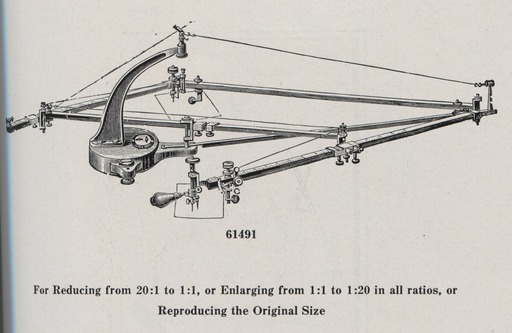
\includegraphics[width=.7\linewidth]{pictures/link-to-elliott-p149-suspended-pantograph-sf0.jpg}
    \caption{Una estructura pantográfica que transmite el movimiento de un punto al siguiente \cite{PantographContext}.}
    \label{fig:estrucutra_pantografica}
\end{figure}

El hecho de que que la estructura del brazo sea pantográfica permite controlar todas las articulaciones mediante motores ubicados en la base. Esto es de especial importancia ya que hace posible que las articulaciones finales no carguen con el peso de los motores, permitiendo emplear materiales como el plástico para la construcción de la estructura y, además, dando capacidad al brazo para levantar cargas más pesadas.

Otro beneficio derivado de la ubicación de los motores en la base es la alta estabilidad del brazo, ya que siendo estos los componentes más pesados y estando ubicados en la base se consigue un centro de gravedad muy cercano a la superficie de apoyo, permitiendo así un amplio rango de movimientos.

Otra característica a destacar es que debido a la estructura pantográfica, el \textit{end--effector} mantiene siempre un ángulo perpendicular con la superficie de apoyo del brazo. Esto supone, por un lado, perder ciertos grados de libertad pero por otro, simplifica la estructura y abarata el coste de producción.